% THIS DOCUMENT IS TAILORED TO REQUIREMENTS FOR SCIENTIFIC COMPUTING.  IT SHOULDN'T
% BE USED FOR NON-SCIENTIFIC COMPUTING PROJECTS
\documentclass[12pt]{article}

\usepackage{amsmath, mathtools}
\usepackage{amsfonts}
\usepackage{amssymb}
\usepackage{graphicx}
\usepackage{colortbl}
\usepackage{xr}
\usepackage{hyperref}
\usepackage{longtable}
\usepackage{xfrac}
\usepackage{tabularx}
\usepackage{float}
\usepackage{booktabs}
\usepackage{caption}
\usepackage{pdflscape}
\usepackage{afterpage}

\usepackage[round]{natbib}

%\usepackage{refcheck}

\hypersetup{
    bookmarks=true,         % show bookmarks bar?
      colorlinks=true,       % false: boxed links; true: colored links
    linkcolor=red,          % color of internal links (change box color with linkbordercolor)
    citecolor=green,        % color of links to bibliography
    filecolor=magenta,      % color of file links
    urlcolor=cyan           % color of external links
}

%% Comments

\usepackage{color}

\newif\ifcomments\commentstrue %displays comments
%\newif\ifcomments\commentsfalse %so that comments do not display

\ifcomments
\newcommand{\authornote}[3]{\textcolor{#1}{[#3 ---#2]}}
\newcommand{\todo}[1]{\textcolor{red}{[TODO: #1]}}
\else
\newcommand{\authornote}[3]{}
\newcommand{\todo}[1]{}
\fi

\newcommand{\wss}[1]{\authornote{blue}{SS}{#1}} 
\newcommand{\plt}[1]{\authornote{magenta}{TPLT}{#1}} %For explanation of the template
\newcommand{\an}[1]{\authornote{cyan}{Author}{#1}}

%% Common Parts

\newcommand{\progname}{OAR} % PUT YOUR PROGRAM NAME HERE
\newcommand{\authname}{Hunter Ceranic} % AUTHOR NAMES                  

\usepackage{hyperref}
    \hypersetup{colorlinks=true, linkcolor=blue, citecolor=blue, filecolor=blue,
                urlcolor=blue, unicode=false}
    \urlstyle{same}
                                


% For easy change of table widths
\newcommand{\colZwidth}{1.0\textwidth}
\newcommand{\colAwidth}{0.13\textwidth}
\newcommand{\colBwidth}{0.82\textwidth}
\newcommand{\colCwidth}{0.1\textwidth}
\newcommand{\colDwidth}{0.05\textwidth}
\newcommand{\colEwidth}{0.8\textwidth}
\newcommand{\colFwidth}{0.17\textwidth}
\newcommand{\colGwidth}{0.5\textwidth}
\newcommand{\colHwidth}{0.28\textwidth}

% Used so that cross-references have a meaningful prefix
\newcounter{defnum} %Definition Number
\newcommand{\dthedefnum}{GD\thedefnum}
\newcommand{\dref}[1]{GD\ref{#1}}
\newcounter{datadefnum} %Datadefinition Number
\newcommand{\ddthedatadefnum}{DD\thedatadefnum}
\newcommand{\ddref}[1]{DD\ref{#1}}
\newcounter{theorynum} %Theory Number
\newcommand{\tthetheorynum}{TM\thetheorynum}
\newcommand{\tref}[1]{TM\ref{#1}}
\newcounter{tablenum} %Table Number
\newcommand{\tbthetablenum}{TB\thetablenum}
\newcommand{\tbref}[1]{TB\ref{#1}}
\newcounter{assumpnum} %Assumption Number
\newcommand{\atheassumpnum}{A\theassumpnum}
\newcommand{\aref}[1]{A\ref{#1}}
\newcounter{goalnum} %Goal Number
\newcommand{\gthegoalnum}{GS\thegoalnum}
\newcommand{\gsref}[1]{GS\ref{#1}}
\newcounter{instnum} %Instance Number
\newcommand{\itheinstnum}{IM\theinstnum}
\newcommand{\iref}[1]{IM\ref{#1}}
\newcounter{reqnum} %Requirement Number
\newcommand{\rthereqnum}{R\thereqnum}
\newcommand{\rref}[1]{R\ref{#1}}
\newcounter{nfrnum} %NFR Number
\newcommand{\rthenfrnum}{NFR\thenfrnum}
\newcommand{\nfrref}[1]{NFR\ref{#1}}
\newcounter{lcnum} %Likely change number
\newcommand{\lthelcnum}{LC\thelcnum}
\newcommand{\lcref}[1]{LC\ref{#1}}

\usepackage{fullpage}

\newcommand{\deftheory}[9][Not Applicable]
{
\newpage
\noindent \rule{\textwidth}{0.5mm}

\paragraph{RefName: } \textbf{#2} \phantomsection 
\label{#2}

\paragraph{Label:} #3

\noindent \rule{\textwidth}{0.5mm}

\paragraph{Equation:}

#4

\paragraph{Description:}

#5

\paragraph{Notes:}

#6

\paragraph{Source:}

#7

\paragraph{Ref.\ By:}

#8

\paragraph{Preconditions for \hyperref[#2]{#2}:}
\label{#2_precond}

#9

\paragraph{Derivation for \hyperref[#2]{#2}:}
\label{#2_deriv}

#1

\noindent \rule{\textwidth}{0.5mm}

}

\begin{document}

\title{Software Requirements Specification for \progname: OAR - Optical Alphabet Recognition} 
\author{Hunter Ceranic}
\date{February 5, 2024}
	
\maketitle

~\newpage

\pagenumbering{roman}

\tableofcontents

~\newpage

\section*{Revision History}

\begin{tabularx}{\textwidth}{p{3cm}p{2cm}X}
\toprule {\bf Date} & {\bf Version} & {\bf Notes}\\
\midrule
February 5, 2024 & 1.0 & Initial Version\\
\bottomrule
\end{tabularx}

~\\

~\newpage

\section{Reference Material}

This section records information for easy reference.

\subsection{Table of Units}

Throughout this document SI (Syst\`{e}me International d'Unit\'{e}s) is employed
as the unit system.  In addition to the basic units, several derived units are
used as described below.  For each unit, the symbol is given followed by a
description of the unit and the SI name.
~\newline

\renewcommand{\arraystretch}{1.2}
%\begin{table}[ht]
  \noindent \begin{tabular}{l l l} 
    \toprule		
    \textbf{symbol} & \textbf{unit} & \textbf{SI}\\
    \midrule 
    px & pixel & picture element\\
  \end{tabular}
  %	\caption{Provide a caption}
%\end{table}

\subsection{Table of Symbols}

The table that follows summarizes the symbols used in this document along with
their units.  The choice of symbols was made to be consistent with the heat
transfer literature and with existing documentation for solar water heating
systems.  The symbols are listed in alphabetical order.

\renewcommand{\arraystretch}{1.2}
%\noindent \begin{tabularx}{1.0\textwidth}{l l X}
\noindent \begin{longtable*}{l l p{12cm}} \toprule
\textbf{symbol} & \textbf{unit} & \textbf{description}\\
\midrule 
$\mathbf{x}_{n \times m}$ & Pixel & Matrix representing pixels of the input image with n rows and m columns, 
\\
$\mathbf{y}_{n \times m}$ & Unitless & Matrix representing the probability values of the pixels of the actual label of the input image
\\
$\mathbf{\hat{y}}_{n \times m}$ & Unitless & Matrix representing the probability values of the pixels of the predicted label of the input image
\\
$\mathbf{z}_{n \times m}$ & Unitless & Matrix representing the combination of pixels from the input image and weights and biaseses, used in the Predicted Label Matrix $\mathbf{\hat{y}}$
\\
$x_{i,j}$ & Unitless & An entry in the input matrix $\mathbf{x}$ (at i, j) which represents the level of intensity of the pixel
\\
$\mathbf{w}_{m \times n}$ & Unitless & Matrix of weights that is used by the classifier model with m rows and n columns
\\
$\mathbf{b}_{n \times m}$ & Unitless & Matrix of biases that is used by the classifier model with n rows and m columns
\\
$\lambda$ & Unitless & Regularization Parameter that affects flexibilty/variance of the model
\\
$\alpha$ & Unitless & Learning rate of classifier model
\\
$\sigma$ & Unitless & Represents the Sigmoid Function
\\
$L$ & Unitless & Represents the Log Loss Function
\\
\bottomrule
\end{longtable*}

\subsection{Abbreviations and Acronyms}

\renewcommand{\arraystretch}{1.2}
\begin{tabular}{l l} 
  \toprule		
  \textbf{symbol} & \textbf{description}\\
  \midrule 
  2D & Two Dimensional\\
  A & Assumption\\
  DD & Data Definition\\
  GD & General Definition\\
  GS & Goal Statement\\
  IM & Instance Model\\
  LC & Likely Change\\
  PS & Physical System Description\\
  R & Requirement\\
  SRS & Software Requirements Specification\\
  TM & Theoretical Model\\
  OAR & Optical Alphabet Recognition\\
  \bottomrule
\end{tabular}\\

\subsection{Mathematical Notation}

In this project documentation variables which represent matrices are indicated by bolded letters (ie. $\mathbf{x}$), whereas
all other variables are represented by regular printed letters.


\newpage

\pagenumbering{arabic}

\section{Introduction}

Images often contain important information to be used in many different modern applications. One such type 
of information that can be contained within images are readable characters, and the motivation for the Optical Alphabet 
Recognition project is to create a system from scratch, that can classify upper-case English letter characters characters accurately.
More information about the problem itself can be found within the Problem Statement document. Furthermore, a foundational goal of
this project is to be useful for educating people about the fundamentals of image classification.

The following section is an overview of the Software Requirement Specifications for the OAR project, specifically outlining the 
purpose of the document, the scope of the requirements, characteristics of the intended reader, and the organization of the 
document.

\subsection{Purpose of Document}

The purpose of this SRS document is to establish and clearly communicate the requirements, limitations, definitions, and models, 
in regards to the OAR project. This document will also serve as basis for reference for the rest of the documents 
supporting the project. 

\subsection{Scope of Requirements} 

The scope for this project is constrained to the recognition of images of handwritten and printed capital-letter English
alphabet characters, in their correct orientations. This does not include hand-written cursive letters.
See the assumptions section (Section 4.2.1) for further details.

\subsection{Characteristics of Intended Reader} \label{sec_IntendedReader}

Readers of this document are intended to have a basic level understanding of 2D image 
processing techniques (equivalent to a standard undergraduate course on machine learning). However, readers with
a prerequisite of at least level one university mathematics knowledge (specifically including matrix linear algebra) will
be able to understand and follow most of the concepts in the document, as the project is also intended to be a useful tools
for learning about image processing.

\subsection{Organization of Document}

  This SRS document contains an introduction to the problem being addressed by the software,
  and the overarching goals of the project. It is to be used as reference for readers based on the
  SRS template by \citet{SmithAndLai2005, SmithEtAl2007}. The scope, terminology, definitions
  and models used in the project are outlined, and more details about the specifics of the problem and the explored
  solution are presented. Requirements, potential future changes and traceability information are also defined.

\section{General System Description}

This section provides general information about the system.  It identifies the
interfaces between the system and its environment, describes the user
characteristics and lists the system constraints.  

\subsection{System Context}

\begin{figure}[h!]
\begin{center}
 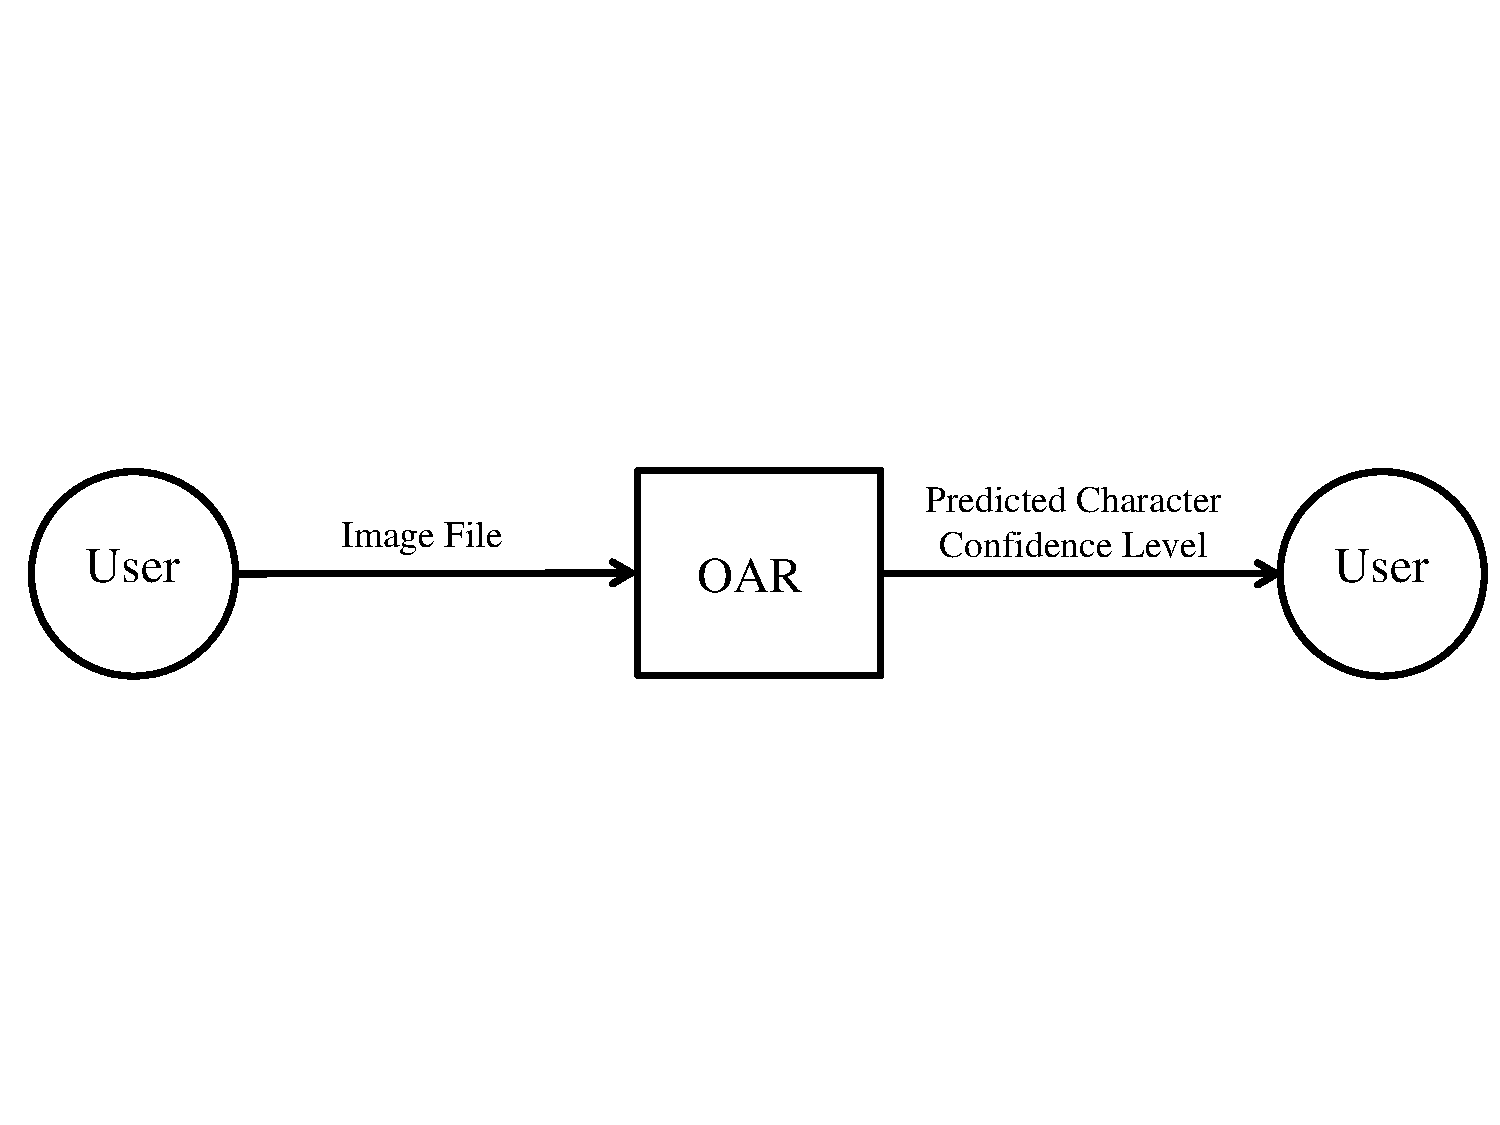
\includegraphics[width=0.6\textwidth]{SystemContextFigure}
\caption{System Context}
\label{Fig_SystemContext} 
\end{center}
\end{figure}


\begin{itemize}
\item User Responsibilities:
\begin{itemize}
\item Provide an image of a character to the program in the proper orientation.
\item Be able to interact with the software program using a keyboard, computer mouse, and monitor.
\item Run the software on a system with the capabilities to sufficently process computer graphics.
\end{itemize}
\item OAR Responsibilities:
\begin{itemize}
\item Provide the ability to load or change image files to be classified.
\item Detect and warn about invalid or corrupt image files, upon input.
\item Display the confidence in the result of classified characters.
\item Provide a user interface which is able to take user input at anytime, with minimal down time where the program is unresponsive.
\end{itemize}
\end{itemize}

\subsection{User Characteristics} \label{SecUserCharacteristics}

The end user of the OAR software is anyone who can use character recognition software or wants to learn about it. This may include 
the intended readers of this document (as described in Section 2.3), however none of those reader requirements are neccessary 
to use the software.

\subsection{System Constraints}

The only real world design constraint for this project is that all input images must have the character in their proper legible
orientation.

\section{Specific System Description}

This section first presents the problem description, which gives a high-level
view of the problem to be solved.  This is followed by the solution characteristics
specification, which presents the assumptions, theories, definitions and finally
the instance models.  

\subsection{Problem Description} \label{Sec_pd}

OAR is intended to classify the characters in images according to their corresponding English language
alphabet characters. It should be able to do this and communicate to users the confidence level in how correctly it 
classified the image.

\subsubsection{Terminology and  Definitions}

This subsection provides a list of terms that are used in the subsequent
sections and their meaning, with the purpose of reducing ambiguity and making it
easier to correctly understand the requirements:

\begin{itemize}

\item Classification: A method of assigning pre-existing labels to processed images.
\item Confidence Level: The probability that the label assigned to an image was correctly identified.
\item Image: A representation of visual information that can be represented by a 2D matrix where each entry represents a pixel with an intensity value.
\item Intensity: The value of a pixel representing it's grayscale colour, on a scale from 0 (which represents black) to 255 (which represents white).
\item Label: A value which associates the result of image classification with a real world category, such as English alphabet letters.
\item Normalization: Altering the aspect ratio and scale of images to some arbitrarily set standard, \cite{Karandish2022}.


\end{itemize}

\subsubsection{Physical System Description} \label{sec_phySystDescrip}

The physical system of OAR, as shown in Figure 2,
includes the following elements:

\begin{itemize}

\item[PS1:] The image that is being input.

\begin{figure}[h!]
  \begin{center}
   
\includegraphics[width=0.6\textwidth]{physicalsystempreprocessing}
  \caption{A sample input image depicting the letter A}
  \label{Fig_PSPreproccessing} 
  \end{center}
  \end{figure}

  To maintain consistency within the software the images will be normalized to some set of n$\times$m pixels such that
  the trained model can classify any given input image. The physical representation of what this resizing will look like
  is seen in Figure 3.

  \begin{figure}[h!]
    \begin{center}
     
\includegraphics[width=0.6\textwidth]{physicalsystem}
    \caption{A sample input image depicting the letter A, after being processed}
    \label{Fig_PS} 
    \end{center}
    \end{figure}


\end{itemize}

\subsubsection{Goal Statements}

\noindent Given an input image, the goal statements are:

\begin{itemize}

\item[GS\refstepcounter{goalnum}\thegoalnum \label{GS1}:] Reprocess the image such that classifying
calculations can be performed on the image.

\item[GS\refstepcounter{goalnum}\thegoalnum \label{GS2}:] Calculate and display the predicted 
corresponding character label for the unknown character in the image.

 \item[GS\refstepcounter{goalnum}\thegoalnum \label{GS3}:] Calculate and display the confidence level that
 the predicted label is correct.

\end{itemize}

\subsection{Solution Characteristics Specification}

This section provides the assumptions, theoretical models, instance models, general definitions,
and data constraints. The information in this section is intended to reduce ambiguity about the project and 
to present the problem in clear mathethematical or logical terms.

The instance models that govern the OAR porject are presented in
Subsection~\ref{sec_instance}.  The information to understand the meaning of the
instance models and their derivation is also presented, so that the instance
models can be verified.

\subsubsection{Assumptions} \label{sec_assumpt}


This section simplifies the original problem and helps in developing the
theoretical model by filling in the missing information for the physical system.
The numbers given in the square brackets refer to the theoretical model [TM],
general definition [GD], data definition [DD], instance model [IM], or likely
change [LC], in which the respective assumption is used.

\begin{itemize}

\item[A\refstepcounter{assumpnum}\theassumpnum \label{A1}:] Normalization, required by \tref{TM2}, as 
well as any other image processing performed before classification calculations, as described in \gsref{GS1}, 
will be performed by supporting libraries.
\item[A\refstepcounter{assumpnum}\theassumpnum \label{A2}:] The dataset used for training the software model
as described by \iref{Train}, will only contain labels of capital letter characters.
\item[A\refstepcounter{assumpnum}\theassumpnum \label{A3}:] The dataset used for training the software model
as described by \iref{Train}, will contain an even spread of every label that can be identified by the porgram.
\item[A\refstepcounter{assumpnum}\theassumpnum \label{A4}:] All input images will be properly oriented so that 
they are legible by the program prior to being input.

\end{itemize}

\subsubsection{Theoretical Models}\label{sec_theoretical}

This section focuses on the general equations and laws that OAR is based
on.  

~\newline

\noindent
\begin{minipage}{\textwidth}
\renewcommand*{\arraystretch}{1.5}
\begin{tabular}{| p{\colAwidth} | p{\colBwidth}|}
\hline
\rowcolor[gray]{0.9}
Number& TM\refstepcounter{theorynum}\thetheorynum \label{TM1}\\
\hline
Label &\bf Sigmoid Function \\
\hline
% Units&$MLt^{-3}T^0$\\
% \hline
Equation & $ \sigma(z) = \frac{1}{1 + e^{-z}} $ \\
\hline
Description &
The sigmoid function takes input $z$ and returns a value between 0 and 1. This function will be used to calculate
the confidence level of the predicted value, to satisfy \gsref{GS3}.
\\
\hline
Notes & The value of $z$ can be a scalar or matrix.
\\
\hline
  Source & \cite{Turin2020}\\
  \hline
  Ref.\ By & \dref{GD_sig}\\
  \hline
\end{tabular}
\end{minipage}\\

~\newline

\noindent
\begin{minipage}{\textwidth}
\renewcommand*{\arraystretch}{1.5}
\begin{tabular}{| p{\colAwidth} | p{\colBwidth}|}
\hline
\rowcolor[gray]{0.9}
Number& TM\refstepcounter{theorynum}\thetheorynum \label{TM2}\\
\hline
Label &\bf Log Loss Function \\
\hline
% Units&$MLt^{-3}T^0$\\
% \hline
Equation & $ L_{(y,\hat{y})} = -\frac{1}{n} \cdot \sum_{i = 1}^{n} (y_i \cdot \log(\hat{y}_i) + (1 - y_i) \cdot \log(1 - \hat{y}_i)) $ \\
\hline
Description &
$y$ represents the actual label value \\
& $\hat{y}$ represents the predicted label value \\
& $n$ is the total number of input values \\
& $i$ is the current step in the summation \\
& \[
    L_{\hat{y}} = 
    \begin{cases}
    -\log(\hat{y}) & \text{, if } y = 1\\
    -\log(1 - \hat{y}) & \text{, if } y = 0
    \end{cases}
\]\\
& This function utilizes the properties of the natural logarithm to determine how similar the actual value $y$ is to the 
predicted value $\hat{y}$. \\

\hline
Notes & The values of $y$ and $\hat{y}$ can be scalar or matrices, but they must be the of the same size (see \aref{A1}).
\\
\hline
  Source & \cite{Turin2020} \\
  \hline
  Ref.\ By & \aref{A1}, \dref{GD_sig}, \dref{GD_gradw}, \dref{GD_gradb}, \iref{Train}\\
  \hline
\end{tabular}
\end{minipage}\\

~\newline

\noindent
\begin{minipage}{\textwidth}
\renewcommand*{\arraystretch}{1.5}
\begin{tabular}{| p{\colAwidth} | p{\colBwidth}|}
\hline
\rowcolor[gray]{0.9}
Number& TM\refstepcounter{theorynum}\thetheorynum \label{TM3}\\
\hline
Label &\bf Chain Rule \\
\hline
% Units&$MLt^{-3}T^0$\\
% \hline
Equation & $\frac{d}{{dx}}\left[ {f\left( u \right)} \right] = \frac{d}{{du}}\left[ {f\left( u \right)} \right]\frac{{du}}{{dx}}$ \\
\hline
Description &

This formula is used to derive the composition of two differentiable functions.
\\
\hline
  Source & \cite{Turin2020}\\
  \hline
  Ref.\ By & \dref{GD_gradw}, \dref{GD_gradb}\\
  \hline
\end{tabular}
\end{minipage}\\

~\newline

\subsubsection{General Definitions}\label{sec_gendef}

This section collects the laws and equations that will be used in building the
instance models.

~\newline

\noindent
\begin{minipage}{\textwidth}
\renewcommand*{\arraystretch}{1.5}
\begin{tabular}{| p{\colAwidth} | p{\colBwidth}|}
\hline
\rowcolor[gray]{0.9}
Number& GD\refstepcounter{defnum}\thedefnum \label{GD_sig}\\
\hline
Label &\bf Sigmoid Function with Input Image and Weights \\
\hline
% Units&$MLt^{-3}T^0$\\
% \hline
SI Units&Unitless\\
\hline
Equation&$ \mathbf{\hat{y}} = \sigma(z) = \frac{1}{1 + (e^{-\mathbf{z}})} \text{, where } z = \mathbf{w}^T \cdot \mathbf{x} + \mathbf{b}$ \\
\hline
Description &
This is a refinement of the Sigmoid function (see \tref{TM1}) to represent how it will be utilized as the basis of the model.
\\
& $\mathbf{x}$ is the input image matrix.\\
& $\mathbf{w}$ is the matrix of weights\\
&$\mathbf{b}$ is the matrix of biases\\
& Note that the predicted value $\mathbf{\hat{y}}$ from \tref{TM2} will be determined from the sigmoid function.\\
\hline
  Source & \cite{Turin2020} \\
  \hline
  Ref.\ By & \dref{GD_gradw}, \dref{GD_gradb}, \iref{Train}, \iref{Test}\\
  \hline
\end{tabular}
\end{minipage}\\

~\newline

\noindent
\begin{minipage}{\textwidth}
\renewcommand*{\arraystretch}{1.5}
\begin{tabular}{| p{\colAwidth} | p{\colBwidth}|}
\hline
\rowcolor[gray]{0.9}
Number& GD\refstepcounter{defnum}\thedefnum \label{GD_gradw}\\
\hline
Label &\bf Gradient of Log Loss Function with respect to $\mathbf{w}$ \\
\hline
% Units&$MLt^{-3}T^0$\\
% \hline
SI Units&Unitless\\
\hline
Equation&$ \nabla_\mathbf{w}  (\mathbf{y}_i \cdot \log(\mathbf{\hat{y}}_i) + (1 - \mathbf{y}_i) \cdot \log(1 - \mathbf{\hat{y}}_i)) = \mathbf{x}_n \cdot (\mathbf{y}_n - \mathbf{\hat{y}}_n)   $\\
\hline
Description &
Here we derive the Log Loss Function with respect to $\mathbf{w}$  using chain rule from \tref{TM3}, with $\mathbf{\hat{y}} $
defined using the Sigmoid Function (see \dref{GD_sig}), so that we can minimize the Log Loss Function to train the model (see \iref{Train}).\\
\hline
  Source & \citet{Turin2020, SharmaLogReg2022} \\
  \hline
  Ref.\ By & \iref{Train}\\
  \hline
\end{tabular}
\end{minipage}\\

~\newline

\noindent
\begin{minipage}{\textwidth}
\renewcommand*{\arraystretch}{1.5}
\begin{tabular}{| p{\colAwidth} | p{\colBwidth}|}
\hline
\rowcolor[gray]{0.9}
Number& GD\refstepcounter{defnum}\thedefnum \label{GD_gradb}\\
\hline
Label &\bf Gradient of Log Loss Function with respect to $\mathbf{b}$ \\
\hline
% Units&$MLt^{-3}T^0$\\
% \hline
SI Units&Unitless\\
\hline
Equation&$ \nabla_\mathbf{b} (\mathbf{y}_i \cdot \log(\mathbf{\hat{y}}_i) + (1 - \mathbf{y}_i) \cdot \log(1 - \mathbf{\hat{y}}_i)) = \mathbf{y}_n - \mathbf{\hat{y}}_n   $\\
\hline
Description &
Here we derive the Log Loss Function with respect to $b$ using chain rule from \tref{TM3}, with $\mathbf{\hat{y}}$ 
defined using the Sigmoid Function (see \dref{GD_sig}), so that we can minimize the Log Loss Function to train the model (see \iref{Train}).\\
\hline
  Source & \citet{Turin2020, SharmaLogReg2022}  \\
  \hline
  Ref.\ By & \iref{Train}\\
  \hline
\end{tabular}
\end{minipage}\\

\subsubsection*{Detailed Derivation of Gradients}

There are three steps to derive the Gradients of the Log Loss Function, using \tref{TM3}. First the outer-most derivative:
\begin{center}
  $$
    [-\mathbf{y} \cdot \log(\mathbf{\hat{y}})]' = \frac{-\mathbf{y}}{\mathbf{\hat{y}}},
  $$
  ~\newline
    and, 
    ~\newline
    $$
    [-(1 - \mathbf{y}) \cdot \log(1 - \mathbf{\hat{y}})]' = \frac{(1 - \mathbf{y})}{(1 - \mathbf{\hat{y}})}, 
    $$
    ~\newline
    which combines to,
    ~\newline
    $$
    \frac{-\mathbf{y}}{\mathbf{\hat{y}}} + \frac{(1 - \mathbf{y})}{(1 - \mathbf{\hat{y}})} = \frac{(\mathbf{\hat{y}} - \mathbf{y})}{(\mathbf{\hat{y}} \cdot (1 - \mathbf{\hat{y}}))}
    $$
\end{center}
Then we take the derivative of $\mathbf{\hat{y}} = \sigma(\mathbf(z))$ using the following identities:
\begin{center}
1. $ 1 - \sigma(z) = 1 - \frac{e^z}{(1 + e^z)} = \frac{1}{(1 + e^z)} = \sigma(-z)$\\
2.$ \frac{d}{dz} \cdot \sigma(z) = \frac{d}{dz} \cdot (1 + e^z)^{-1} = \frac{e^{-z}}{(1 + e^{-z})^2} = \frac{e^{-z}}{(1 + e^{-z})} \cdot \frac{1}{(1 + e^{-z})} = \sigma(-z) \cdot \sigma(z) = (1 - \sigma(z)) \cdot \sigma(z) $
\end{center}
Which gives $ \mathbf{y}_n' = \mathbf{y}_n \cdot (1 - \mathbf{y}_n)$
~\newline
Then finally we take the last derivative in the chain, which is where the gradient derivations differentiate:
\begin{center}
For \dref{GD_gradw}: $ \frac{d}{d\mathbf{w}} \cdot (\mathbf{b} + \mathbf{x}_1 \cdot \mathbf{w}_1 + ... +\mathbf{x}_n \cdot \mathbf{w}_n) = \mathbf{x}_i$ \\
For \dref{GD_gradb}: $\frac{d}{d\mathbf{b}} \cdot (\mathbf{b} + \mathbf{x}_1 \cdot \mathbf{w}_1 + ... +\mathbf{x}_n \cdot \mathbf{w}_n) = 1 $
\end{center}

Then each derivative in the chain is multiplied together for $\nabla_\mathbf{w}$ and $\nabla_b$ respectively, resulting in
the final formulas seen in \dref{GD_gradw} and \dref{GD_gradb}. 


\subsubsection{Data Definitions}\label{sec_datadef}

This section collects and defines all the data needed to build the instance
models. The dimension of each quantity is also given.  
~\newline

\noindent
\begin{minipage}{\textwidth}
\renewcommand*{\arraystretch}{1.5}
\begin{tabular}{| p{\colAwidth} | p{\colBwidth}|}
\hline
\rowcolor[gray]{0.9}
Number& DD\refstepcounter{datadefnum}\thedatadefnum \label{DD1}\\
\hline
Label& \bf Learning Rate\\
\hline
Symbol &$\alpha$\\
\hline
% Units& $Mt^{-3}$\\
% \hline
  SI Units & Unitless\\
  \hline
  Equation& Not Applicable\\
  \hline
  Description & 
                Learning Rate is the value that is used to help the model minimize the Log Loss function effectively at each step.
                While there is no concrete equation to determine the learning rate it is suggested that fine-tuning is done by
                increasing or decreasing the value by a factor of 10.
  \\
  \hline
  Sources& \cite{SharmaRegParm2022} \\
  \hline
  Ref.\ By & \iref{Train}\\
  \hline
\end{tabular}
\end{minipage}\\

~\newline

\noindent
\begin{minipage}{\textwidth}
\renewcommand*{\arraystretch}{1.5}
\begin{tabular}{| p{\colAwidth} | p{\colBwidth}|}
\hline
\rowcolor[gray]{0.9}
Number& DD\refstepcounter{datadefnum}\thedatadefnum \label{DD2}\\
\hline
Label& \bf Regularization Parameter\\
\hline
Symbol &$\lambda$\\
\hline
% Units& $Mt^{-3}$\\
% \hline
  SI Units & Unitless\\
  \hline
  Equation& Not Applicable\\
  \hline
  Description & 
                The regularization parameter is a value that is used to help the model minimize the Log Loss function to reduce
                overfitting. While there is no concrete equation to determine the regularization parameter it is suggested 
                that fine-tuning is done by increasing or decreasing the value by a factor of 10.
  \\
  \hline
  Sources& \cite{SharmaRegParm2022}\\
  \hline
  Ref.\ By & \iref{Train}\\
  \hline
\end{tabular}
\end{minipage}\\


~\newline
\subsubsection{Instance Models} \label{sec_instance}    

This section transforms the problem defined in Section~\ref{Sec_pd} into 
one which is expressed in mathematical terms. It uses concrete symbols defined 
in Section~\ref{sec_datadef} to replace the abstract symbols in the models 
identified in Sections~\ref{sec_theoretical} and~\ref{sec_gendef}.

The goals \gsref{GS2} and \gsref{GS3} are solved by \iref{Test}. \iref{Train} is used 
to train the model so that \iref{Test} can be used reliably and efficiently.

~\newline

%Instance Model 1

\noindent
\begin{minipage}{\textwidth}
\renewcommand*{\arraystretch}{1.5}
\begin{tabular}{| p{\colAwidth} | p{\colBwidth}|}
  \hline
  \rowcolor[gray]{0.9}
  Number& IM\refstepcounter{instnum}\theinstnum \label{Train}\\
  \hline
  Label& \bf Model Training via Gradient Descent\\
  \hline
  Input&$\mathbf{x}_n$, $\mathbf{y}_n$, $\mathbf{\hat{y}}_n = \frac{1}{1 + (e^(\mathbf{w}^T \cdot \mathbf{x} + \mathbf{b}))}, \alpha \text{ from \ddref{DD1}}, \lambda \text{ from \ddref{DD2}}, N$ which is the number of training images\\
  & The input is constrained so that \aref{A2} and \aref{A3} can be satisfied.\\
  \hline
  Output & $\mathbf{w}, \mathbf{b} $ \\
  \hline
  Description &
  Using gradient descent we minimize the Log Loss Function to optimize the weights and biases for better predictions\\
  & This is executed in the following order, over multiple epochs ($t$) to further optimize the values:
  \begin{itemize}
    \item 1. For each set of training images, calculate the following:
    \begin{itemize}
        \item 1.1. $d\mathbf{w}^{(t)} = \mathbf{x}_n \cdot (\mathbf{y}_n - \mathbf{\hat{y}}_n) - \frac{lambda}{N} \cdot \mathbf{w}^{(t)^2} $
        \item 1.2. $d\mathbf{b}^{(t)} = \mathbf{y}_n - \mathbf{\hat{y}}_n$
        \item 1.3. $\mathbf{w}^{(t+1)} = \mathbf{w}^{(t)} + \alpha \cdot d\mathbf{w}^{(t)}$
        \item 1.4. $d\mathbf{b}^{(t+1)} = d\mathbf{b}^{(t)} + \alpha \cdot d\mathbf{b}^{(t)}$
    \end{itemize}
    \item 2. Calculate the Log Loss and test the results using the updated weights.
 \end{itemize}
  \\
  \hline
  Sources & \citet{Turin2020, SharmaLogReg2022} \\
  \hline
  Ref.\ By & \aref{A2}, \aref{A3}, \iref{Test}, \rref{R3}\\
  \hline
\end{tabular}
\end{minipage}\\

~\newline

%Instance Model 2

\noindent
\begin{minipage}{\textwidth}
\renewcommand*{\arraystretch}{1.5}
\begin{tabular}{| p{\colAwidth} | p{\colBwidth}|}
  \hline
  \rowcolor[gray]{0.9}
  Number& IM\refstepcounter{instnum}\theinstnum \label{Test}\\
  \hline
  Label& \bf Label Classification\\
  \hline
  Input&$\mathbf{x}$, $\mathbf{y}_n$, $\mathbf{w}$, $b$\\
  \hline
  Output & $\mathbf{\hat{y}}$, and the string representation of the corresponding predicted label \\
  \hline
  Description &
  Using the optimized weights and biases from \iref{Train} and combining that with an unknown input $\mathbf{x}$ in
  the Sigmoid function (see \dref{GD_sig}), then comparing across the sigmoid values of
  the 26 possible labels, the most likely label can be predicted. In addition the confidence level in the prediction can
  be calculated as the output of the sigmoid function for the related predicted label.
  \\
  \hline
  Sources & \citet{Turin2020, SharmaLogReg2022} \\
  \hline
  Ref.\ By & \rref{R4}, \rref{R5}\\
  \hline
\end{tabular}
\end{minipage}\\
~\newline



\subsubsection{Input Data Constraints} \label{sec_DataConstraints}    

Table~\ref{TblInputVar} shows the data constraints on the input output
variables.  The column for physical constraints gives the physical limitations
on the range of values that can be taken by the variable.  The column for
software constraints restricts the range of inputs to reasonable values.  The
software constraints will be helpful in the design stage for picking suitable
algorithms.  The constraints are conservative, to give the user of the model the
flexibility to experiment with unusual situations.  The column of typical values
is intended to provide a feel for a common scenario.  The uncertainty column
provides an estimate of the confidence with which the physical quantities can be
measured.  This information would be part of the input if one were performing an
uncertainty quantification exercise.

The specification parameters in Table~\ref{TblInputVar} are listed in
Table~\ref{TblSpecParams}.

\begin{table}[!h]
  \caption{Input Variables} \label{TblInputVar}
  \renewcommand{\arraystretch}{1.2}
\noindent \begin{longtable*}{l l l l c} 
  \toprule
  \textbf{Var} & \textbf{Physical Constraints} & \textbf{Software Constraints} &
                             \textbf{Typical Value} & \textbf{Uncertainty}\\
  \midrule 
  $x_{i,j}$& - & ${\text{min }} x_{i,j} \leq x_{i,j} \leq {\text{max }} x_{i,j}$ & 128 & 10\%
  \\
  $\mathbf{x}_{n \times m}^1$& - & ${\text{min }} n, m \leq n, m \leq {\text{max }} n, m$ & $1024 \times 1024$ & 10\%
  \\
  \bottomrule
\end{longtable*}
\end{table}

\noindent 
\begin{description}
\item $^1$ The constraints on the input image matrix are strictly on it's size $n \times m$ not on the matrix itself.
\end{description}

\begin{table}[!h]
\caption{Specification Parameter Values} \label{TblSpecParams}
\renewcommand{\arraystretch}{1.2}
\noindent \begin{longtable*}{l l} 
  \toprule
  \textbf{Var} & \textbf{Value} \\
  \midrule 
  $\text{min } x_{i,j}$ & 0\\
  $\text{max } x_{i,j}$ & 255\\
  $\text{min } n \times m$ & 20 px $\times$ 20px\\
  $\text{max } n \times m$ & 4096 px $\times$ 4096px\\
  \bottomrule
\end{longtable*}
\end{table}

\subsubsection{Properties of a Correct Solution} \label{sec_CorrectSolution}

\noindent
A correct solution must come in the form of one of the 26 possible labels,
\newline{\{A,B,C,D,E,F,G,H,I,J,K,L,M,N,O,P,Q,R,S,T,U,V,W,X,Y,Z\}}, as well as an associated 
confidence level, as a percentage, that the label assigned is correct.

\section{Requirements}

This section provides the functional requirements, the business tasks that the
software is expected to complete, and the nonfunctional requirements, the
qualities that the software is expected to exhibit.

\subsection{Functional Requirements}

\noindent \begin{itemize}

\item[R\refstepcounter{reqnum}\thereqnum \label{R1}:] Accept an input image in the following formats: \begin{itemize}
  \item PNG (Portable Net Graphics)
  \item JPEG (Joint Photographic Experts Group)
  \item BMP (Bitmap)
  \item preloaded training images
\end{itemize}

\item[R\refstepcounter{reqnum}\thereqnum \label{R2}:] Process the image such that the calculations
needed to be performed by the program can be executed.

\item[R\refstepcounter{reqnum}\thereqnum \label{R3}:] Provide a trained model that can accurately classify images using
26 different labels (see \iref{Train}).

\item[R\refstepcounter{reqnum}\thereqnum \label{R4}:] Calculate and display the classified label for the input image (see \iref{Test}).

\item[R\refstepcounter{reqnum}\thereqnum \label{R5}:] Calculate and display the confidence level that the assigned
label is correct (see \iref{Test}).

\end{itemize}

\subsection{Nonfunctional Requirements}

\noindent \begin{itemize}

\item[NFR\refstepcounter{nfrnum}\thenfrnum \label{NFR1}:]
  \textbf{Accuracy} The accuracy of the computed label confidence should be consistent enough that the results 
  could be considered comparable to other existing solutions for this problem. As such, the accuracy of the model
  on the training data set should be output in the form of a confusion matrix. In addition the confidence level output has to
  be calculated in a similar way to existing solutions so that the output can be verified and compared to other algorithms.

\item[NFR\refstepcounter{nfrnum}\thenfrnum \label{NFR2}:] \textbf{Usability}
  The user should be able to intuitively use the software and understand the output that is displayed.
  To accomplish this the software should be user-friendly, simple, and require little setup. A user survey
  may be conducted to verify the software's percieved usability.

\item[NFR\refstepcounter{nfrnum}\thenfrnum \label{NFR3}:]
  \textbf{Maintainability} The code should be clear and understandable to make further development by other programmers 
  possible with little hassle, as well as to help educate newer programmers as to how image classification works.
  Adding further features, or understanding how the software presently works should not be a difficult task.


\item[NFR\refstepcounter{nfrnum}\thenfrnum \label{NFR4}:]
  \textbf{Portability} The software should be cross-platform (Windows, Linux, MacOS) with little to no setup
  required. This can be in the the form of an executable python-based application.

\end{itemize}

\subsection{Rationale}

The rationale for \aref{A1} to limit the scope of the project to the problem of classification, rather then including
other problems such as normalization, given that \gsref{GS2} and \gsref{GS3} are the goals of the software which return an output
to the user.

\section{Likely Changes}

The changes listed below are likely to be implemented as the software is developed further.

\noindent \begin{itemize}

\item[LC\refstepcounter{lcnum}\thelcnum\label{LC1}:] Expand the number of classification labels
to include lower-case English letter alphabet, numerical, and punctuation characters. 
\item[LC\refstepcounter{lcnum}\thelcnum\label{LC2}:] Allow the user to specify whether the image is being
input from a camera or from a pre-existing file on their system.

\end{itemize}

\section{Unlikely Changes}    

\noindent \begin{itemize}

\item[LC\refstepcounter{lcnum}\thelcnum\label{LC3}:] Expand the functionality of the program to classify
whole English words and sentences instead of just individual characters.
\item[LC\refstepcounter{lcnum}\thelcnum\label{LC4}:] Provide the choice of different image classification algorithms.


\end{itemize}

\section{Traceability Matrices and Graphs}

The purpose of the traceability matrices is to provide easy references on what
has to be additionally modified if a certain component is changed.  Every time a
component is changed, the items in the column of that component that are marked
with an ``X'' may have to be modified as well.  Table~\ref{Table:trace} shows the
dependencies of theoretical models, general definitions, data definitions, and
instance models with each other. Table~\ref{Table:R_trace} shows the
dependencies of instance models, requirements, and data constraints on each
other. Table~\ref{Table:A_trace} shows the dependencies of theoretical models,
general definitions, data definitions, instance models, and likely changes on
the assumptions.

\afterpage{
\begin{landscape}
\begin{table}[h!]
\centering
\begin{tabular}{|c|c|c|c|c|}
\hline
	& \aref{A1}& \aref{A2}& \aref{A3}& \aref{A4} \\
\hline
\tref{TM1}        & & & &  \\ \hline
\tref{TM2}        & & & &  \\ \hline
\tref{TM3}        & & & & \\ \hline
\dref{GD_sig}        & & & &  \\ \hline
\dref{GD_gradw}        & & & & \\ \hline
\dref{GD_gradb}       & & & & \\ \hline
\ddref{DD1}       & & & &  \\ \hline
\ddref{DD2}       & & & X &  \\ \hline
\iref{Train}       & X & X & X & X \\ \hline
\iref{Test}        & X & & & X \\ \hline
\lcref{LC1}        & & X & X & X \\ \hline
\lcref{LC2}        & & & & X \\ \hline
\lcref{LC3}        & & X & X & X \\ \hline
\lcref{LC4}       & X & & & X \\
\hline
\end{tabular}
\caption{Traceability Matrix Showing the Connections Between Assumptions and Other Items}
\label{Table:A_trace}
\end{table}
\end{landscape}
}

\begin{table}[h!]
\centering
\begin{tabular}{|c|c|c|c|c|c|c|c|c|c|c|}
\hline        
	& \tref{TM1}& \tref{TM2}& \tref{TM3}& \dref{GD_sig}& \dref{GD_gradw} & \dref{GD_gradb}& \ddref{DD1} & \ddref{DD2}& \iref{Train}& \iref{Test}\\
\hline
\tref{TM1}     & & & & X & X & X & & & X & X \\ \hline
\tref{TM2}     & & & & & X & X & & & X &  \\ \hline
\tref{TM3}     & & & & & X & X & & & X &  \\ \hline
\dref{GD_sig}     & & & & & & & & & X & X \\ \hline
\dref{GD_gradw}     & & & & & & & & & X &  \\ \hline
\dref{GD_gradb}    & & & & & & & & & X &  \\ \hline
\ddref{DD1}    & & & & & & & & & X &  \\ \hline
\ddref{DD2}    & & & & & & & & & X &  \\ \hline
\iref{Train}    & & & & & & & & & &  \\ \hline
\iref{Test}     & & & & & & & & & & X \\ 
\hline
\end{tabular}
\caption{Traceability Matrix Showing the Connections Between Items of Different Sections}
\label{Table:trace}
\end{table}

\begin{table}[h!]
\centering
\begin{tabular}{|c|c|c|c|c|c|c|c|c|c|c|c|}
\hline
	& \iref{Train}& \iref{Test}& \rref{R1}& \rref{R2}& \rref{R3}& \rref{R4}& \rref{R5} & \nfrref{NFR1} & \nfrref{NFR2} & \nfrref{NFR3} & \nfrref{NFR4} \\
\hline
\iref{Train}    & & & & & & & & & & &  \\ \hline
\iref{Test}    & & & & & & & & & & &  \\ \hline
\rref{R1}     & & & & & & & & & & & \\ \hline
\rref{R2}     & & & & & & & & & & & \\ \hline
\rref{R3}     & X & & & & & & & & & &\\ \hline
\rref{R4}     & & X & & & & & & & & &\\ \hline
\rref{R5}     & & X & & & & & & & & &\\ \hline
\nfrref{NFR1}   & & X & & & & & & & & & \\ \hline
\nfrref{NFR2}   & & X & X & & & & & & & &\\ \hline 
\nfrref{NFR3}   & & & & & & & & & & &\\ \hline
\nfrref{NFR4}   & & & & & & & & & & &\\ 
\hline
\end{tabular}
\caption{Traceability Matrix Showing the Connections Between Requirements and Instance Models}
\label{Table:R_trace}
\end{table}

\section{Values of Auxiliary Constants}
There are no auxiliary constants defined so this section is not applicable for this project.

\newpage

\bibliographystyle {plainnat}
\bibliography {../../refs/References}

\end{document}